%!TEX root =  ../final-report.tex
%
% Chapters are setup to start on a new page. The short version of that title appears in square brackets. This is used for the
% table of contents listing. The long version of the title has a command "\setstretch{0.5}" in order to reduce the line
% spacing in the title and then the title text.
\chapter{Vector Network Analyzer}
\label{sec:VNA}

The vector network analyzer is a key component of the S-Parameter Data Acquisition (SPDAQ) system since it is the actual
instrument that measures the S-Parameters of the grain storage unit.

% Sections will automatically be numbered by LaTeX.
\section{Harware Specifications}

In order to implement a practical system that would be ideally used by agriculturalists such as farmers, the VNA had to be
portable yet affordable. Lab quality VNAs are very expensive, usually costing tens of thousands of dollars, and therefore
cannot be used for the SPDAQ system. Due to the fairly low frequencies being transmitted and received from the antennas
within the grain storage unit, the VNA can be more affordable than those usually found in a lab.  On top of these main
specifications of a compact, low-costing VNA, the analyzer had to be a two port system so it is capable of S11 and S12
measurements for the microwave imaging of the grain bin,as well as being capable of measuring within the frequency range of a typical grain bin,and can offer a good dynamic range.  Table \ref{table:vna} shows the exact specifications required for the SPDAQ system to be effective.
\clearpage{}
\begin{table}[!h]
\centering
\caption{VNA Requirements \cite{vnaspecs}}
\label{table:vna}
\begin{tabular}{|l|l|}
\hline
Frequency Range & 70 MHz - 100 MHz 			\\ \hline
Dynamic Range   & ≥ 10 dB          			\\ \hline
System Type     & 2-port with S11 and S12 	\\ \hline
Budget   		& \textless \$1000		\\ \hline
\end{tabular}
\end{table}

These criteria help facilitate in the decision of selecting the MiniVNA Pro (MVP) by Mini Radio Solutions which offers a more affordable and portable solution for the VNA component of the SPDAQ system.

\begin{table}[!h]
\centering
\caption{miniVNA PRO Specifications}
\label{table:mvp}
\begin{tabular}{|l|l|}
\hline
Frequency Range & 0.1 MHz - 200 MHz                                                                             \\ \hline
Dynamic Range   & \begin{tabular}[c]{@{}l@{}}90 dB in Transmission mode\\ 50 dB in Reflection mode\end{tabular} \\ \hline
System Type     & 2-port with S11 and S12                                                                       \\ \hline
Cost            & \$549.95 + taxes and fees							\\ \hline
\end{tabular}
\end{table}

As shown in Table \ref{table:mvp}, the MVP meets all the main VNA requirements for the SPDAQ system which made it a valid solution
for the VNA component.
\clearpage{}
\section{Calibration and Testing}

To ensure that the MVP meets our system’s standards, results measured from the MVP were compared to the more high-tech VNAs
in the Electromagnetic Imaging Lab (EIL) that are normally used for the imaging data.  The MVP is first calibrated using the calibration tool provided by the EIL and calibration files are created using the MVP software, which is shown in Figure \ref{fig:calib}.
\newline
\begin{figure}[!ht]
\begin{center}
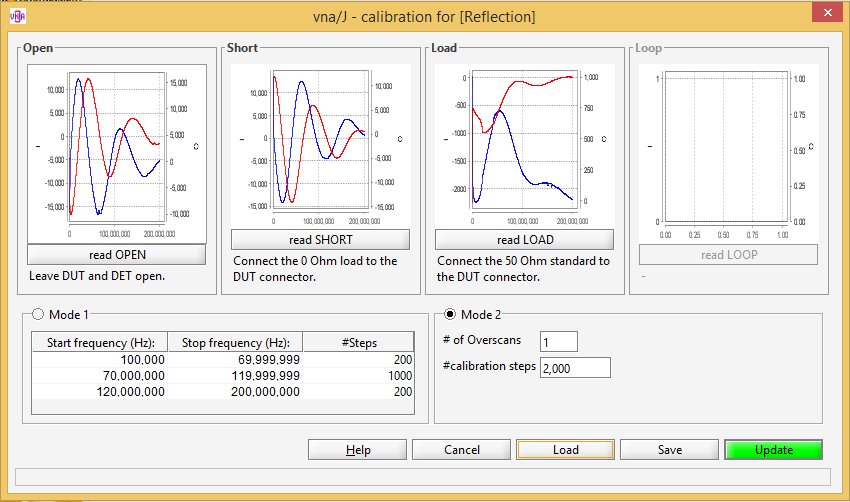
\includegraphics[width=4.9in]{./images/calib.png}
\caption{miniVNA PRO calibration software.}
\label{fig:calib}
\end{center}
\end{figure}

The S11 measurement of the miniVNA PRO was then compared to the S11 measurement of the EIL VNA in order to verify the calibration was performed correctly on the miniVNA PRO. The RF Switch module provided by the EIL was used as a load. The S11 output of the RF Switch transfer function is shown in Figure \ref{fig:real} and \ref{fig:imag} for both the EIL VNA and the miniVNA PRO. Both the real and imaginary part of the S11 measurement are fairly similar with a slight discrepancy in the real part of S11 in the miniVNA PRO which may be due to the calibration kit used with the miniVNA Pro since the kit was designed for the EIL VNAs. 
With fairly accurate results, the MVP gave us confidence in using it for the SPDAQ system. 

\begin{figure}[!ht]
\begin{center}
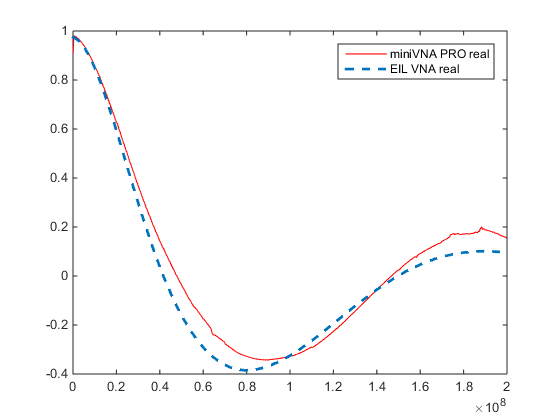
\includegraphics[width=3.8in]{./images/real.png}
\caption{S11 measurement(real) for both VNAS.}
\label{fig:real}
\end{center}
\end{figure}

\begin{figure}[!ht]
\begin{center}
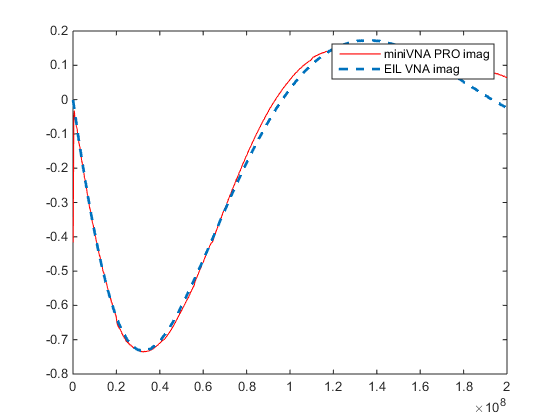
\includegraphics[width=3.8in]{./images/imag.png}
\caption{miniVNA PRO open port measurement in reflection mode.}
\label{fig:imag}
\end{center}
\end{figure}

\clearpage{}
\section{miniVNA PRO Software}

The MVP was designed to be software-defined and the manufacturer did not have any indications that they will make this device
open source. This forced our team to go ahead with the manufacturer’s software in order to use the MVP despite the slow read
times of each measurement.
\newline

\begin{figure}[h]
\begin{center}
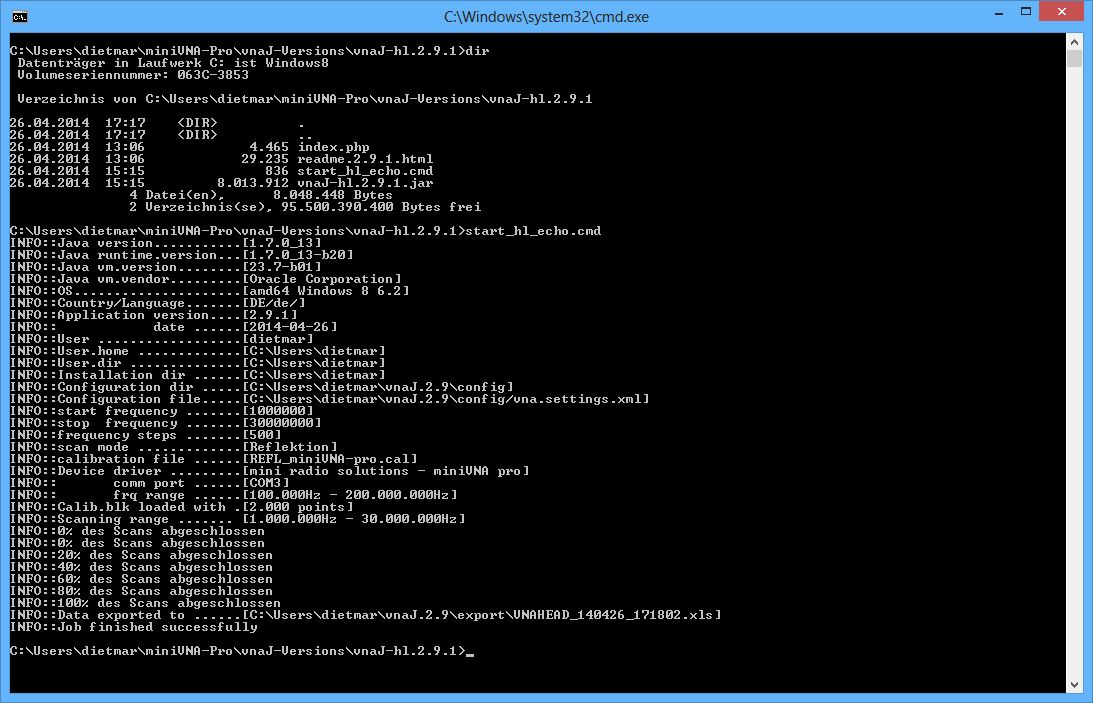
\includegraphics[width=4.5in]{./images/cli.jpg}
\caption{miniVNA PRO Software Output}
\label{fig:cli}
\end{center}
\end{figure}

The MVP’s software used for the SPDAQ system is the ‘vnaJ-hl.3.1.3.jar’ file [3] that runs on a headless system (no graphical
user interface). When the jar file is executed with the specified parameters (frequency start, stop and steps), the MVP takes
the readings and exports them to a CSV file (the file type is specified within the parameters of the jar file).  An example
output of the MVP’s software running through a command line interface (CLI) is shown in Figure \ref{fig:cli}.



\chapter{Microprocessor}
\label{sec:software}

% Sections will automatically be numbered by LaTeX.

\section{Hardware Integration}

Due to the software limitation of the MiniVNA Pro (MVP), a microprocessor was required to run the MVP’s software. This is
where the Raspberry Pi 2 (RPi 2) was chosen.  The RPi 2 microprocessor will be used to control both the RF Multiplexer and
MiniVNA Pro (MVP) of the S-Parameter Data Acquisition (SPDAQ) system.  The specifications of the RPi 2 are shown in Table
\ref{table:RPi2}.

\begin{table}[h]
\centering
\caption{Raspberry Pi 2 Specifications \cite{RPi2}}
\label{table:RPi2}
\begin{tabular}{|l|l|}
\hline
Processor & 900Mhz quad-core ARM Cortex-A7 CPU 	\\ \hline
RAM       & 1GB									\\ \hline
USB Ports & 4                                  	\\ \hline
GPIO Pins & 40				\\ \hline
\end{tabular}
\end{table}

The RPi2 offers enough USB ports to connect the RF Multiplexer (RF Mux) and MVP.  As well, the RPi2 offers GPIO pins, which will be used to integrate user interface (UI) features for the user to have better control of the system.  Such UI features that were
implemented with the RPi2 was a button to run the SPDAQ’s software when pressed and a LED indicator to allow the user to know
when the program is ready for the user to press the button.  A circuit is shown in Figure \ref{fig:button} that displays the button
and LED connection to the appropriate GPIO pins on the RPi2 (see Appendix \ref{appendix:rpi2} for Raspberry Pi 2 Pinout Configuration).

\begin{figure}[h]
\begin{center}
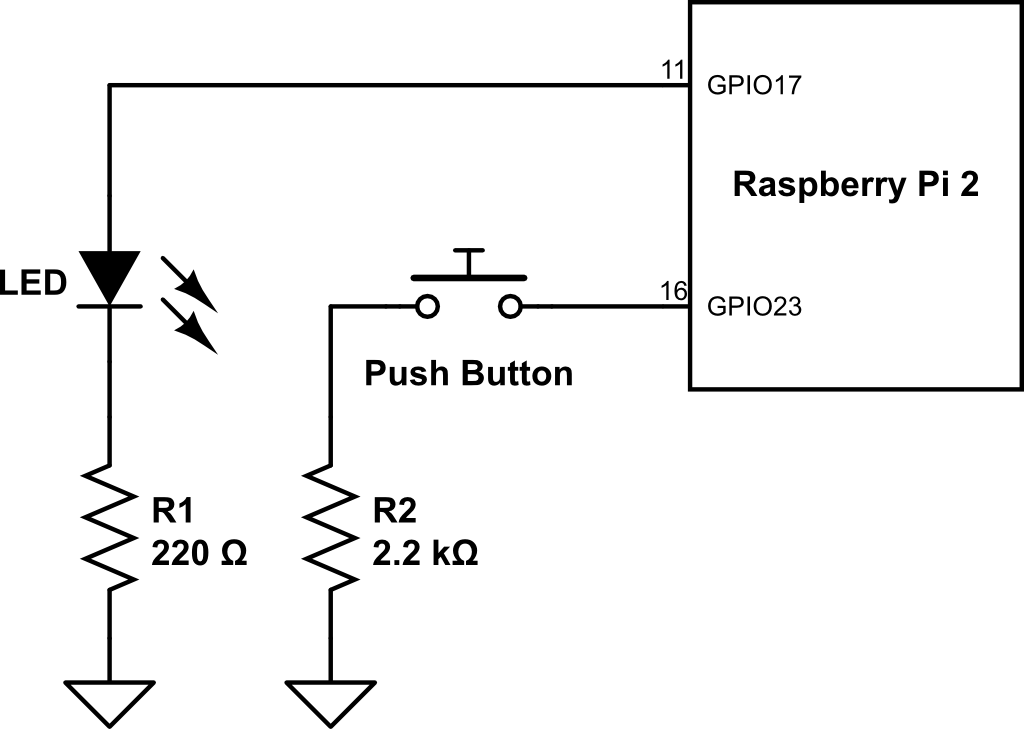
\includegraphics[width=3.8in]{./images/rpi2.png}
\caption{LED and Button Circuit}
\label{fig:button}
\end{center}
\end{figure}

Initially, the SPDAQ system was designed around the Raspberry Pi Model B+ but due to the new release of the RPi 2 in
February, 2015, the decision to upgrade seem obvious with the faster processor at the same low cost of 39.99 CAD + shipping
that the old Raspberry Pi Model B+ was priced at.  The hardware upgrade helped greatly improve the software run times down to
16s per measurement to ~5s per measurement.  Boot up times for the system also greatly reduced to 6s from 15s.

\section{Software Design and Integration}

Arch Linux was installed onto the RPi 2 due to its minimal architecture. It is a lightweight operating system (OS) that is
text-based with no GUI making it very quick to boot up.  Since the SPDAQ system has no need for a GUI and the software that
will be running on the RPi 2 did not require much to run, the Arch Linux OS provided a great solution for our system.

For the SPDAQ system, there are four main processes that the system is required to run: Initialization, Data Acquisition,
Post-Data Processing, and Remote Data Accessing. The order of all these processes and procedures that run on the
microprocessor are shown in Figure \ref{fig:procs}.

\begin{figure}[h]
\begin{center}
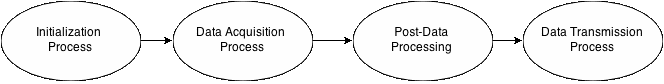
\includegraphics[width=5.4in]{./images/procs.png}
\caption{S-Parameter Data Acquisition system processes.}
\label{fig:procs}
\end{center}
\end{figure}

\subsection{Initialization Process}

The initialization process requires the user to interact with the system to power on and start the other processes that are
executed by a shell script.  The procedure is as follows:

\begin{enumerate}
\item Power on the S-Parameter Data Acquisition (SPDAQ) system by connecting the RPi2 to a power source.
\item Once booted up (allow approximately 7s), the user can now press the push button to execute a shell script that will start the data acquisition process.
\end{enumerate}

\subsection{Data Acquisition Process}

In this process, the RPi 2 will control both the RF Multiplexer to switch the antennas between transmitter and receiver as
well triggering the MVP to execute a sweep to obtain S-Parameters of the Grain Bin.  The Data Acquisition Process runs
through an N-number antenna array collecting the S-parameter data from the grain bin through the use of the MVP, which
exports a CSV file per sweep.  Each antenna will act as a transmitter and will loop through all n number of antennas acting
as a receiver, which results in an N x N number of measurements.  This will also result in N x N number of exported data
files from the MVP due to its software limitations.  These data files are exported to
/root/vnaJ.3.1.3/export directory of the RPi2.  A flow chart of the Data
Acquisition Process is shown in Figure \ref{fig:switch} which outlines this procedure.

\begin{figure}[h]
\begin{center}
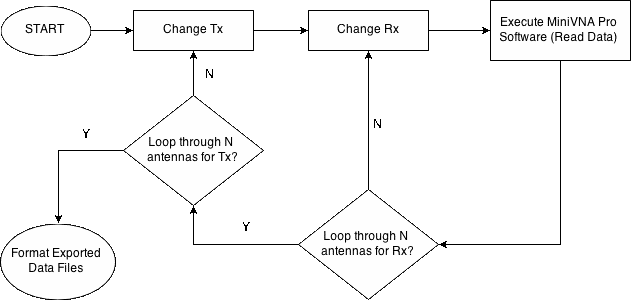
\includegraphics[width=5in]{./images/switch.png}
\caption{Flow chart of the Data Acquisition Process.}
\label{fig:switch}
\end{center}
\end{figure}

\subsection{Post-Data Processing}

Post-Data Processing procedure is executed by the shell script after the Data Acquisition Process is done.  In this process,
the exported CSV files from the MVP are reformatted to a single data file, which the user can access for further processing
such as microwave imaging analysis of the grain bin.  The exported CSV files are located in the
/root/vnaJ.3.1/export directory with the filename format of
$gbin_{tx}{rx}.csv$ where “{tx}” and “{rx}” are the 2-digit transmitter and receiver antenna number, respectively, within the
array that the MVP measured from. The MVP exports the data as transmission loss in dB and transmission phase (degrees), which
is S12 in polar form, however Cartesian complex form is required for post-analysis and therefore a small calculation is
required prior to writing to file. The calculations performed are described below:
\clearpage{}
\noindent
The MVP provides its data as so, 
\\$Transmission Loss (TL)=20\log_{10}|S12| Transmission Phase= \theta$
\noindent
The desired data form is as so, $S12=a+bi$
\noindent
Variables a and b are calculated as shown, 
\\$a=|S12|\cos\theta b=|S12|\sin\theta where,|S12|= 10^{(TL/20)}$

Once the S12 data is calculated to Cartesian complex format, it is then written to a file called “sp.dat” which is located in
/root/grainbin/output/ directory.  The format of the file is shown as:

\begin{verbatim}
Tx	Rx	Probe	    S12 Real	S12 Imaginary (repeating for all frequency steps)
\end{verbatim}

Where Tx is the transmitter antenna number and Rx is the receiver antenna number, which is then followed by the S12 real and
imaginary data in succession for all 100 frequency steps.  A flow chart of the Post-Data Processing procedure is shown in Figure
\ref{fig:pdp}.


\begin{figure}[h]
\begin{center}
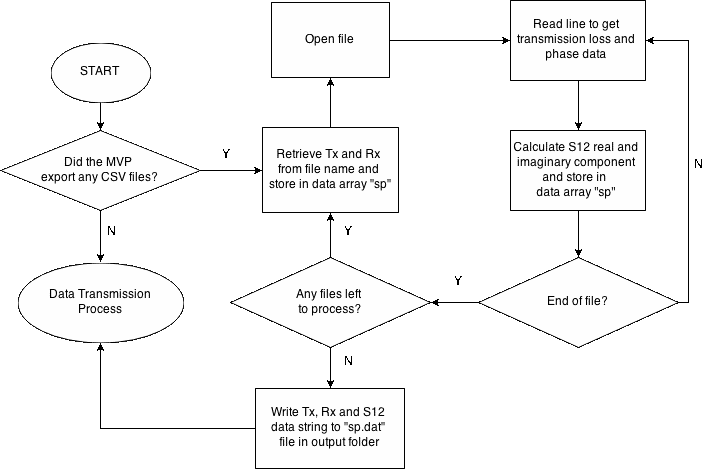
\includegraphics[width=5in]{./images/pdp.png}
\caption{Flow Chart of Post-Data Processing
Procedure.}
\label{fig:pdp}
\end{center}
\end{figure}

\subsection{Data Transmission Process}

The “sp.dat” file contains all of the S-parameters of the grain storage unit and this file will be accessible to the user
through the cloud if an Internet connection is present.  The shell script will execute the data upload process after the
Post-Data Processing is complete in which it executes a command in Linux that triggers an upload of the specific file to
Dropbox.

Dropbox is a widely used cloud storage service that anyone can register for free for basic cloud storage space. This service
can be accessed online remotely from the users own PC through the many interfaces that Dropbox offers (ex. website, computer
software, etc.), which makes it very convenient for the user to retrieve the data from the SDAS and therefore was selected
for our system.  Appendix \ref{appendix:dropbox} instructs how a user can unlink or link a specific Dropbox account onto the RPi2 as well as
additional commands.

However, if the SPDAQ system is unable to connect to the Internet to upload the data file, the user can still manually
retrieve the data through the following methods:

\begin{enumerate}
\item Ejecting the micro-SD card located underneath the RPi2 in which the file is stored on.
\item SFTP with the RPi2 through an Ethernet connection with another device.
\begin{itemize}
\item The RPi2 is assigned a static IP address for the user to SSH and SFTP in order to communicate with it. That static IP address is: \textit{192.168.2.23}.  Once SFTP establishes a connection, executing the command, \textit{“get /root/grainbin/output/sp.dat”} will transfer the file over to the users remote device.
\end{itemize}
\end{enumerate}

\section{Software Setup and Configuration}

This chapter section details the software setup and configuration on the RPi2 to run the SPDAQ software. The purpose of this
section is to help a user recreate the SPDAQ software on the RPi2 in the case of any software error or corruption or to
simply modify specific software parameters to tailor to the user’s needs.

\subsection{Prerequisites} The RPi2 is setup with a username and password.  The default login information for Arch Linux is
the following:

\begin{verbatim}
Username: root 
Password: root
\end{verbatim}

However for security purposes, the password was changed to 'gbin2015' with the same username.
\newline
In order for the RPi2 software processes to function, certain files need to be included on the RPi2 stored in the directory
/root/grainbin. A list of these files is shown in Table \ref{table:files}

\begin{table}[h]
\centering
\caption{Required files in the /root/grainbin directory of the Raspberry Pi 2.}
\label{table:files}
\resizebox{\textwidth}{!}{%
\begin{tabular}{|l|l|}
\hline
\textbf{File}		& \textbf{Description} 																						\\ \hline
vnaJ-hl.3.1.3.jar   & miniVNA PRO headless software 																			\\ \hline
gbin.sh 			& shell script t run all of the SPDAQ processes (see Appendix \ref{appendix:gbinsh}) 								\\ \hline
dropbox-uploader.sh & Dropbox shell script to upload "sp.dat" file to a linked Dropbox account on the RPi2 (see Appendix \ref{appendix:dropbox})   																										\\ \hline
put2str.exe         & processes the exported CSV files from the miniVNA PRO (see Appendix \ref{appendix:put2str}) 						\\ \hline
button.py 			& button and LED function on the Raspberry Pi 2 (see Appendix \ref{appendix:button})	\\ \hline
\end{tabular}
}
\end{table}

Specific packages also need to be installed onto the RPi2 for the files to run properly on the Arch Linux OS. The following
commands shown in Table \ref{table:pkg} can be executed on the RPi2 terminal with Arch Linux installed.  Ensure that the RPi2 is connected to the Internet in order to download these packages.

\begin{table}[h]
\centering
\caption{Required packages to be installed on Arch Linux OS running on the Raspberry Pi 2.}
\label{table:pkg}
\begin{tabular}{|l|l|}
\hline
\textbf{Command}				& \textbf{Description} 				\\ \hline
pacman –S jdk7-openjdk			& Java package 						\\ \hline
pacman –S mono                  & C\# Compiler                     	\\ \hline
pacman –S python-raspberry-gpio & Raspberry Pi GPIO Python library	\\ \hline
\end{tabular}
\end{table}

Once the packages are installed, the MVP’s software requires specific directories to be created. These directories are
created when the ‘vnaJ-hl.3.1.3.jar’ file is executed for the first time which can be executed using the following command:

\noindent
\textbf{\textit{ java –Dconfigfile=gbin.xml -Dfstart=70000000 -Dfstop=100000000 -Dfsteps=100 -Dcalfile=gbin.cal -Dscanmode=TRAN -Dexports=csv -jar vnaJ-hl.3.1.3.jar}}

An error will occur due to certain files missing when the command is executed for the first time however the necessary
directories will be created on the /root directory of the RPi2 which includes:
\setlist{noitemsep}
\begin{itemize}
\item /root/vnaJ.3.1/export
\item /root/vnaJ.3.1/calibration
\item /root/vnaJ.3.1/config
\end{itemize}

There are two key files that need to be present for the ‘vnaJ-hl.3.1.3.jar’ file to execute properly.  The first one is the
configuration file “gbin.xml” which can be found in Appendix \ref{appendix:xml}.  The XML file includes the USB port name for the software to
communicate with the MVP. This file must be stored in the /root/vnaJ.3.1/config directory. The second key file is the
calibration file for transmission mode which are created using the ‘vnaJ.3.1.3.jar’ GUI software that must be run on a
separate computer that supports either Mac OS or Windows.  The user should consult the vnaJ software user manual \cite{vnaj} for
details on how these calibration files are created using the ‘vnaJ.3.1.3.jar’ GUI. This calibration file is stored in the
\noindent
\textit{/root/vnaJ.3.1/config} directory.
\newline
The RPi2 is now setup to run the ‘gbin.sh’ shell script that runs the SPDAQ software.   In order to use the button and LED
feature, the python script ‘button.py’ needs to be executed. The simple command “Python button.py” will run the python script
and will listen for the user to press a button to initiate the ‘gbin.sh’ script.  In order to setup the python script
‘button.py’ at bootup, the following command can be entered on the terminal of the RPi2:

\textbf{\textit{crontab –e}}

\noindent 
A file will come up and in this file enter in the line at the very bottom:

\textbf{\textit{@reboot python /root/grainbin/button.py}}

\noindent
Save the file and now the RPi2 will run the python script at bootup, enabling the button and LED function. To connect the LED and push button to the RPi2, review Figure \ref{fig:button} and Appendix \ref{appendix:rpi2} for GPIO pinout on the RPi2. 

\subsection{Configuration Parameters}

\subsubsection{‘gbin.sh’ Parameters}

The 'gbin.sh' shell script file is designed to take 4 parameters that define the number of transmitters and receivers being
used with the SPDAQ system.  The command to run the 'gbin.sh' file through the RPi2 terminal is:

\textbf{\textit{sh gbin.sh \{1\} \{2\}\ \{3\} \{4\}}}

\noindent
The 4 parameters are defined in Table \ref{table:gbinsh}.

\begin{table}[h]
\centering \caption{Parameter definitions for 'gbin.sh'.}
\label{table:gbinsh}
\begin{tabular}{|l|l|}
\hline
\textbf{Parameter} 	& \textbf{Description}             \\ \hline
\{1\}              	& transmitter antenna start number \\ \hline
\{2\}				& transmitter antenna stop number  \\ \hline
\{3\}     			& receiver antenna start number    \\ \hline
\{4\}              	& receiver antenna stop number			\\ \hline
\end{tabular}
\end{table}

An example of this command when using transmitter antennas 1-10 and antennas 11-20 as receiving,

\textbf{\textit{sh gbin.sh 01 10 11 20}}

\subsubsection{miniVNA PRO Software Parameters}

The MVP software is executed within the ‘gbin.sh’ shell script (refer to Appendix  \ref{appendix:gbinsh}) and the parameters can be changed by
changing the following command within that script:

\noindent
\textbf{\textit{java –Dconfigfile=gbin.xml -Dfstart=\{Start\} -Dfstop=\{Stop\} -Dfsteps=\{Steps\} 
\\-Dcalfile=gbin.cal -Dscanmode=TRAN -Dexports=csv -jar vnaJ-hl.3.1.3.jar}}

Where the following parameters are defined in Table \ref{table:vnaj}.

\begin{table}[h]
\centering
\caption{Parameter definitions for miniVNA PRO software command.}
\label{table:vnaj}
\begin{tabular}{|l|l|}
\hline
\textbf{Parameter} 	& \textbf{Description} 			\\ \hline
\{Start\}          	& Frequency range start (Hz) 	\\ \hline
\{Stop\}           	& Frequency range stop (Hz)		\\ \hline
\{Steps\} 			& Number of Frequency steps	\\ \hline
\end{tabular}
\end{table}

\noindent
The command is set within the shell script by default as:

\noindent
\textbf{\textit{java –Dconfigfile=gbin.xml -Dfstart=70000000 -Dfstop=100000000 -Dfsteps= 100
\\-Dcalfile=gbin.cal -Dscanmode=TRAN -Dexports=csv -jar vnaJ-hl.3.1.3.jar }}

\noindent
Where the frequency range is 70-100MHz with 100 steps.  The user can refer to the vnaJ Headless Software Manual
\cite{vnaJ-hl} for additional information.

\chapter{Future Work}

At the moment, the SPDAQ system is at an early stage of development. Our team has developed an Alpha prototype of the SPDAQ
system for hardware and software testing in order to establish a proof of concept for this project. Although our team was
successful in integrating the many hardware and software components for the system, there are still many things that can be improved on to make the system accessible to the general public. Initial designs for the SPDAQ system was to implement a battery operated device however due to project time constraints and project delays, this feature has yet to be implemented but should considered for future iterations. This chapter will explain the possible work that can be
done to advance the current alpha prototype of the SPDAQ system and its individual components.

\section{Software}

As of now, the current software is at its very basic form where a shell script executes the SPDAQ software on the RPi2 with
very little interface for the user to interact with.  The user can edit certain files on the RPi2 in order to modify the
settings which requires root access to the RPi2. This current method requires a good knowledge of the LINUX OS which is not
commonly known by the average user.  By implementing a more advanced GUI, the user can have more control over the SPDAQ
system with an easier method to setup and configure any of the settings of the SPDAQ software.  The GUI can also offer an
easier method for the user to connect the RPi2 to the Internet for cloud services with a use of a Wifi adapter. To improve the software runtime, the use of another VNA that is open source should be considered in newer iterations of the SPDAQ system.

\section{RF Multiplexer Module}

At this stage, the RF Multiplexer component is currently being built and has yet to be tested.  Through our SPDAQ prototype testing, we used an old RF Switch module provided by the EIL for the Alpha build.  The RF Mux module designed by our team offers the same logistics as the RF Switch module provided by the EIL and therefore the upgrade to the newly designed RF Mux model, once manufactured, should be a simple transition.  The work to be done once our RF Mux PCBs arrive will be to solder the RF switch integrated circuits (ICs) and to test with the rest of the SPDAQ Alpa prototype.

\section{Antennna}

The H-field antennas have been designed and tested. For the future, the E-Field antenna design will need to be modified in order to reduce cross-polarization so it can meet the SPDAQ system standards for a grain storage unit.  Once modified, further tests need to be conducted with the antenna integrated with the SPDAQ system.
